\subsection{Probability Density Analysis}
\label{appx-a:ch1:probability-density-analysis}

The details described in this section address the prerequisites for the performed null hypothesis test in Section~\ref{ch1:subsec:probability-density-analysis}.
These steps lie beyond the content of the corresponding chapter, yet have been included for completeness.
Here, each step to condition the raw data for the $t$-test is explained in detail.

The original data is a highly volatile and non-stationary time-series that has a non-gaussian probability distribution.
However, in order to apply the $t$-test, these criteria have to be met.
Data conditioning steps were followed for each dataset that would modify the properties of the time-series without modifying their context.
These steps are listed below and go as follows: First

\begin{enumerate}
	\item the time-series is rescaled using the $\log()$ function, then
	\item the rescaled values is averaged over $N$ samples, then
	\item the averages are split into two distinct sections (one prior to 11am and one after 11am), then
	\item the sections are compared against each other (i.e. by computing the difference), then
	\item the comparison's auto-correlation is computed to check for the presence of self-dependence.
	\begin{enumerate}
		\item If the self-dependence is low enough (i.e. within confidence interval) the $t$-test is executed
		\item otherwise the data is feathered and the auto-correlation is tested again, and
		\item if the results still indicate a self-dependence, then a different $N$ is chosen and the steps are repeated.
	\end{enumerate}
\end{enumerate}

To visualise this procedure, the dataset corresponding to the minimisation of distribution losses, i.e. $\zeta_\text{losses}()$, is presented and the data modifications are explained.
Since the steps apply to all data sets, only one is being presented in this appendix.

\begin{figure}\centering
	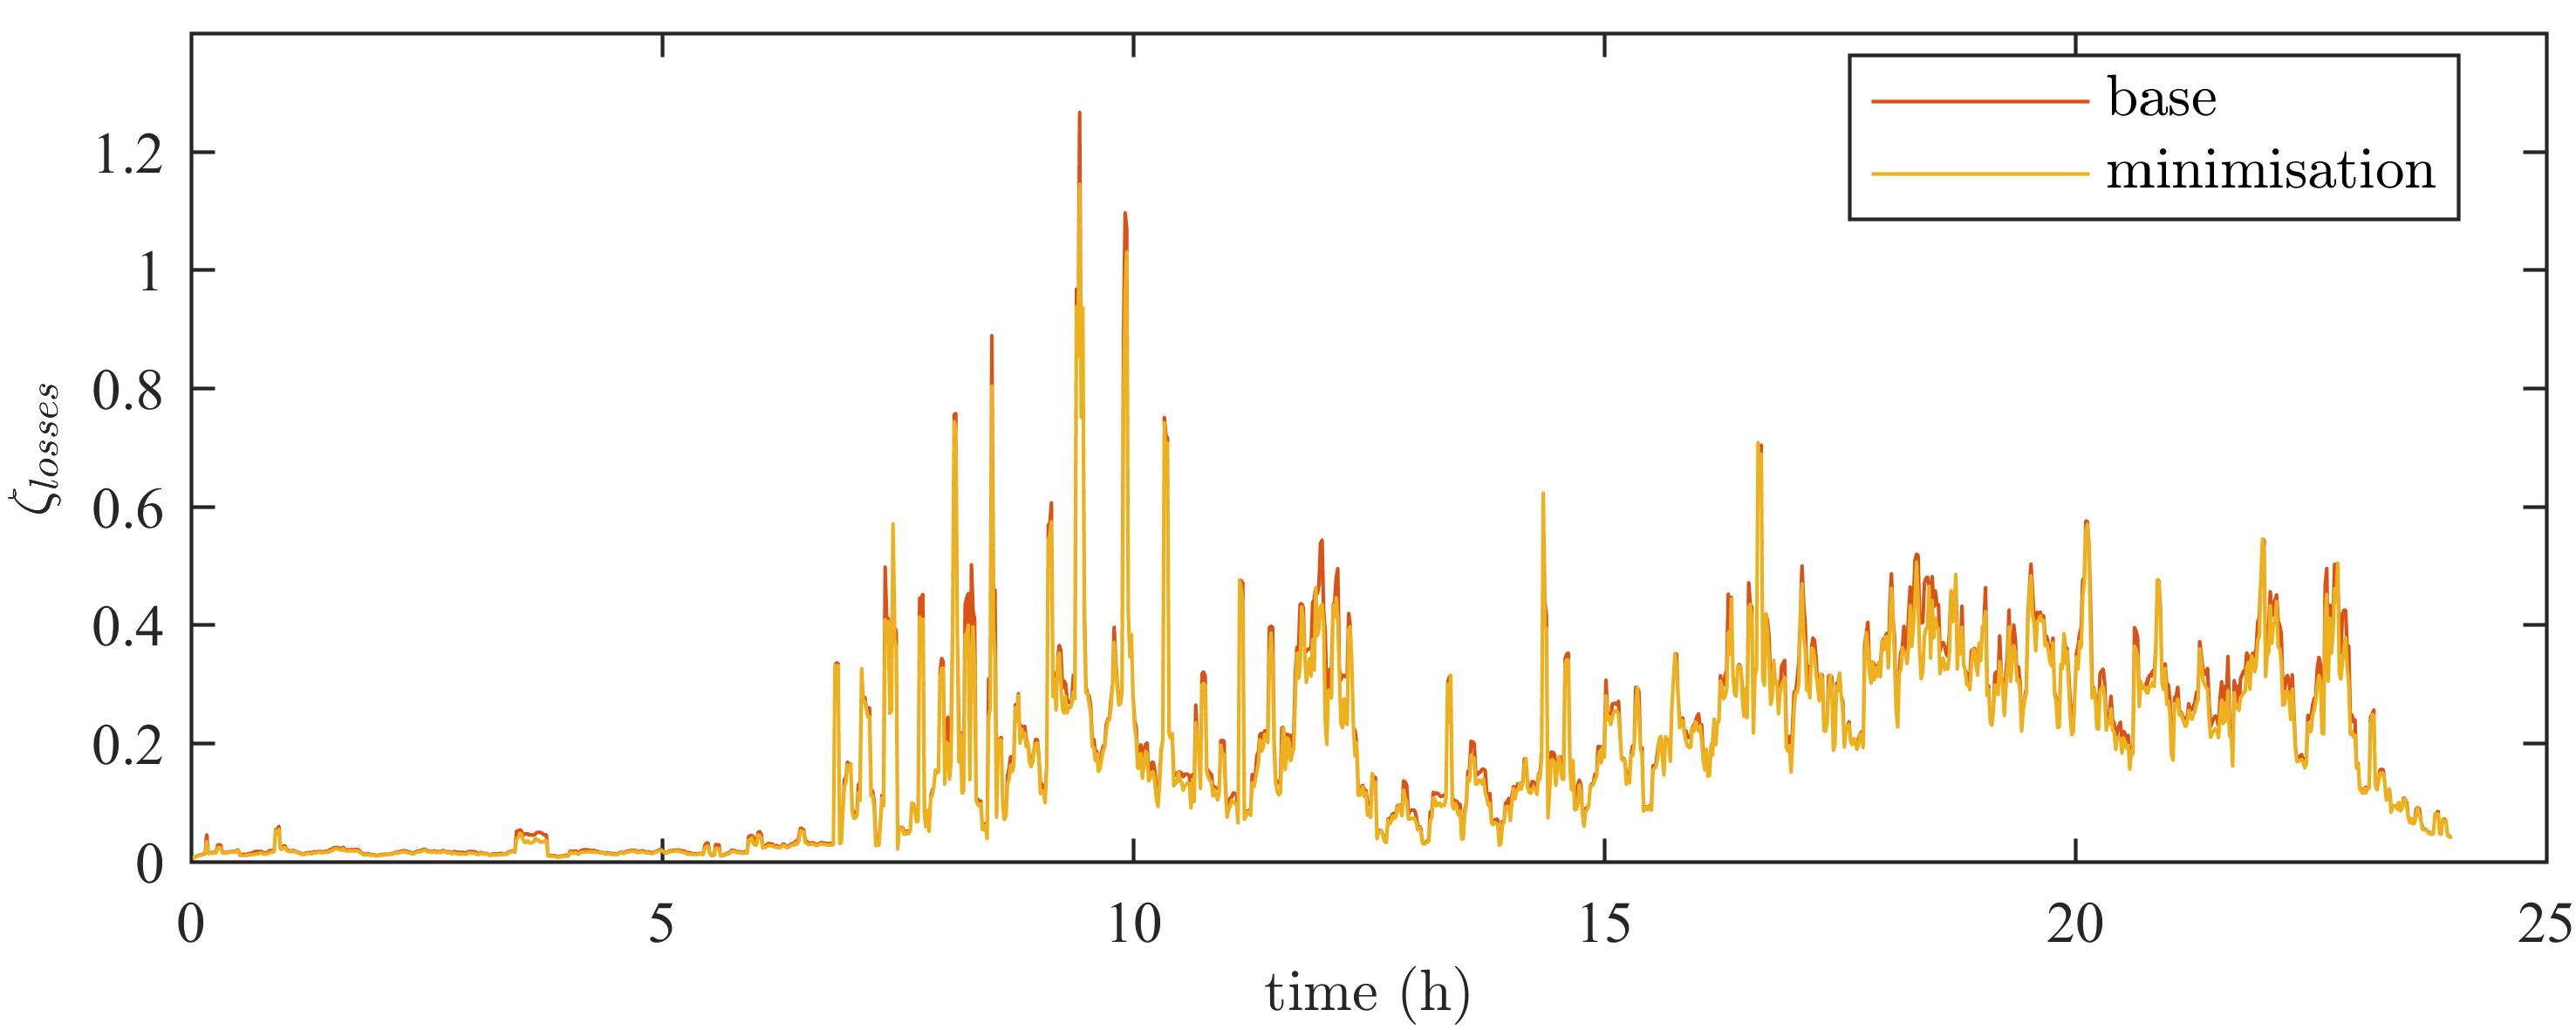
\includegraphics{_appendices/_a1/fig/raw-cost}
	\caption{Raw time-series that are supposed to be compared.}
	\label{appx-a:ch1:fig:raw-data}
\end{figure}

Figure~\ref{appx-a:ch1:fig:raw-data} shows the raw data of the two time-series that are going to be compared in the $t$-test.
Since this data is very spiky and has many values located closely to zero, they are scaled using the $\log()$ function.

\begin{figure}\centering
	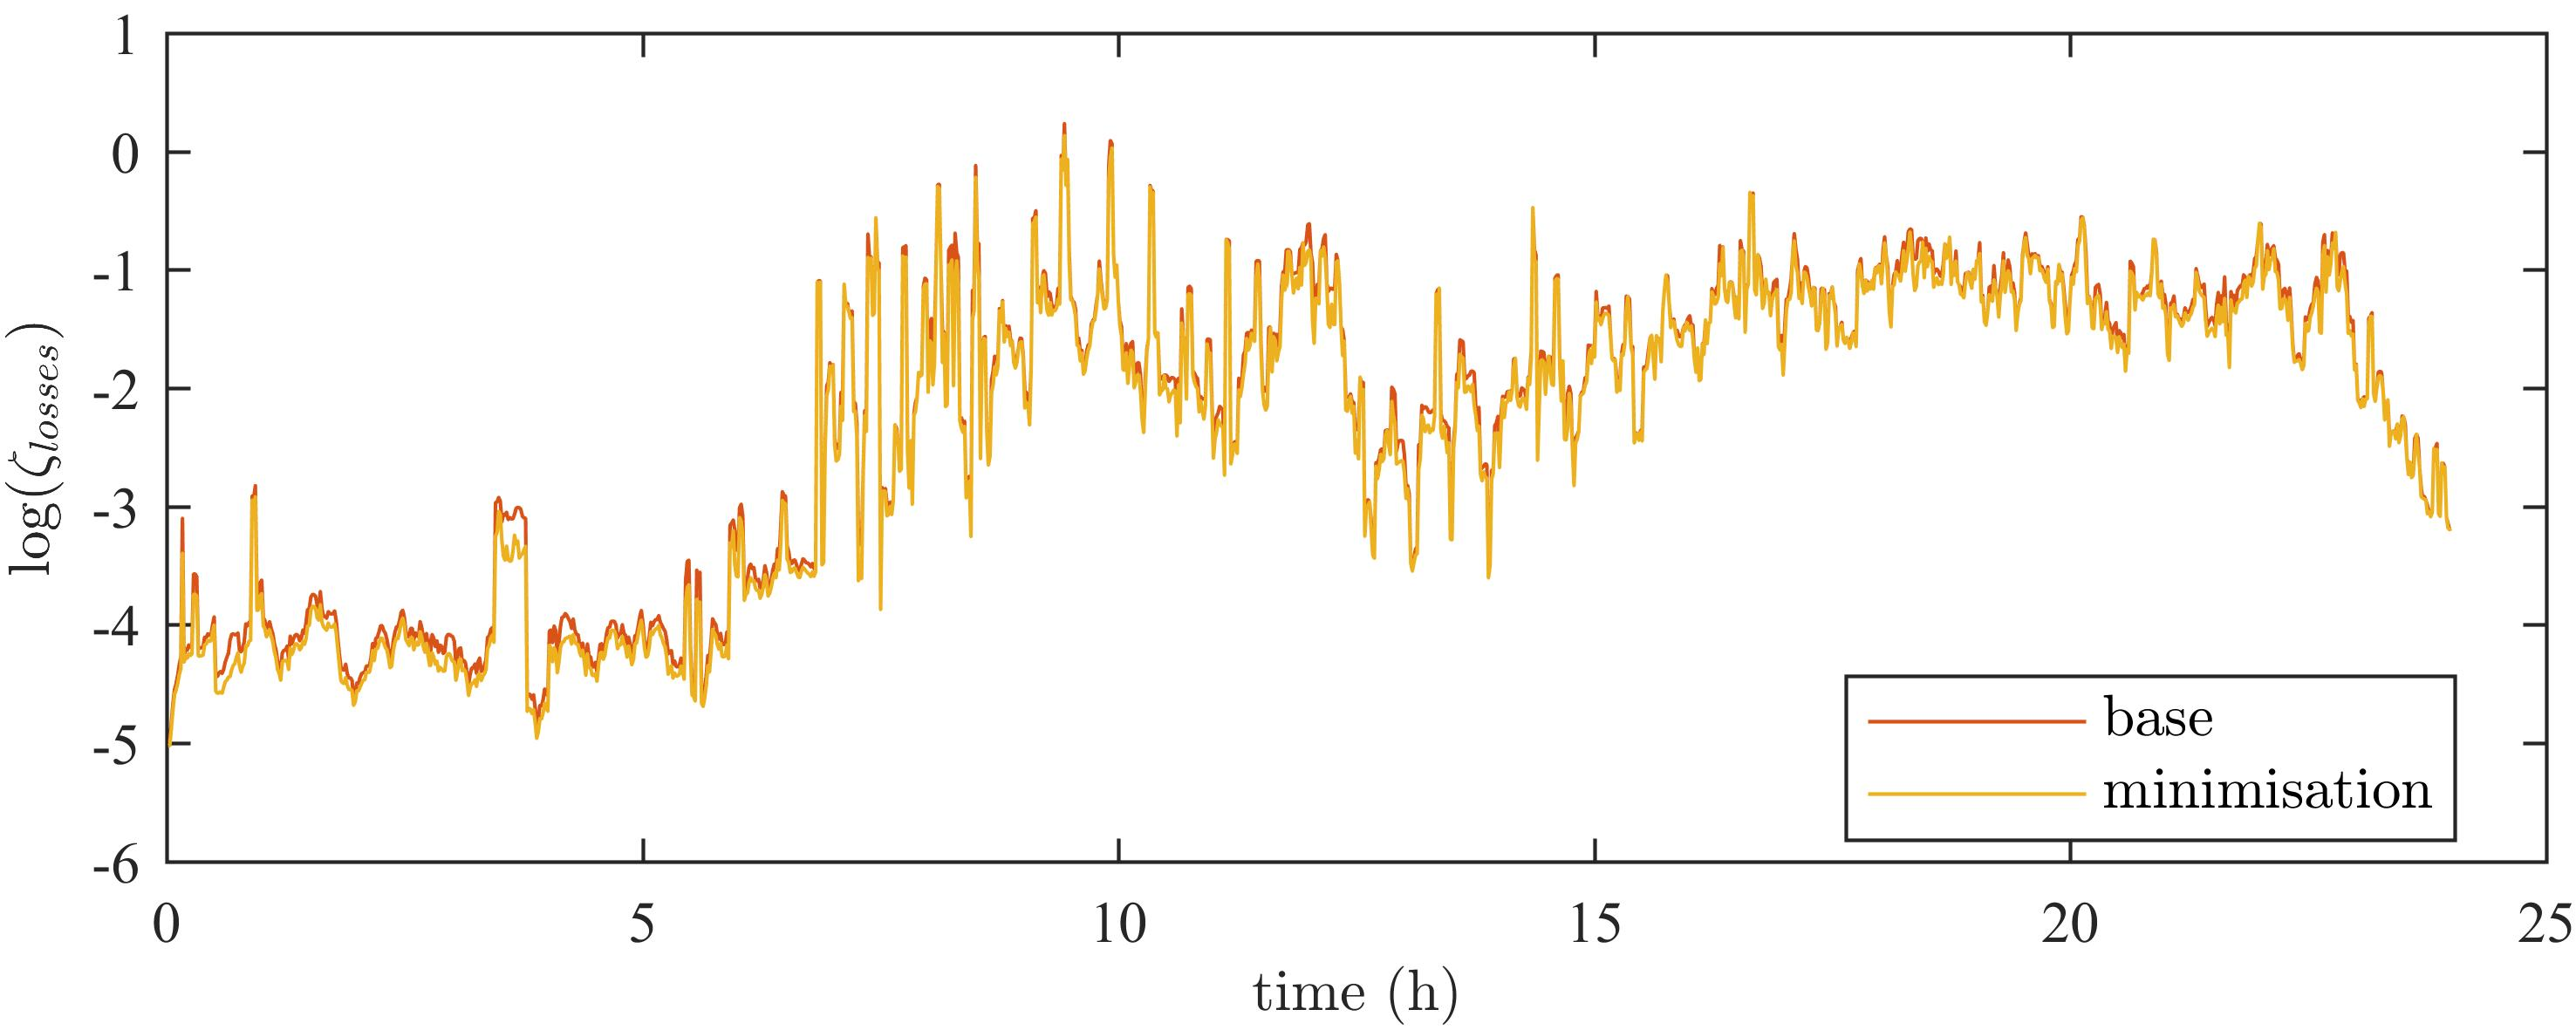
\includegraphics{_appendices/_a1/fig/log-cost}
	\caption{Rescaled time-series that are supposed to be compared.}
	\label{appx-a:ch1:fig:log-data}
\end{figure}

Figure~\ref{appx-a:ch1:fig:log-data} shows this rescaled cost.
It can be observed how differences, like the increase in load during the morning hours, has become more apparent.
Nonetheless, this data is still volatile and is averaged over $N$ values.

\begin{figure}\centering
	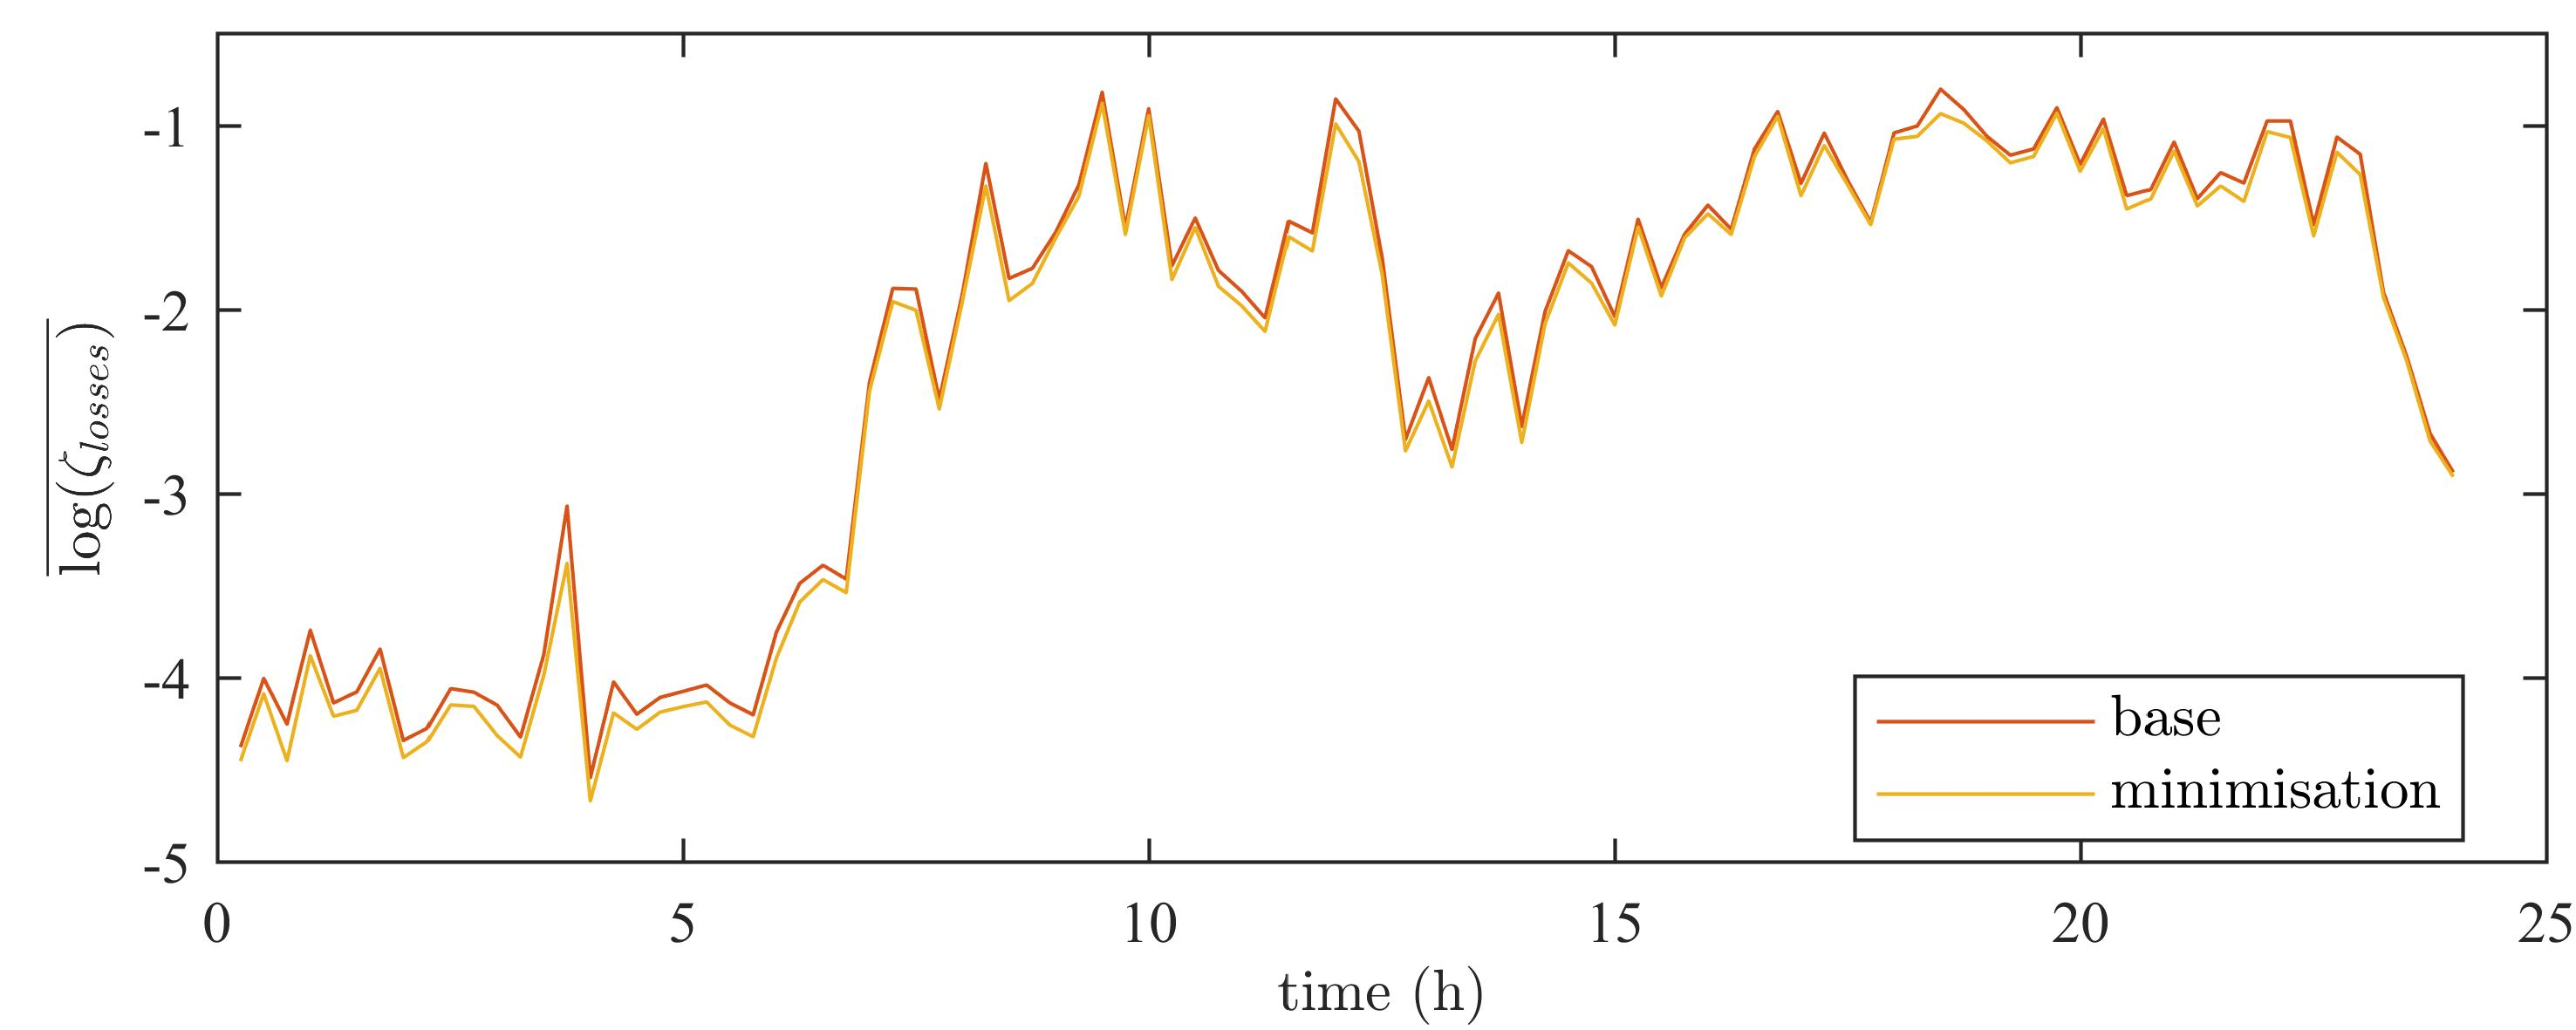
\includegraphics{_appendices/_a1/fig/averaged-log-cost}
	\caption{Averaged log-scaled time-series.}
	\label{appx-a:ch1:fig:averaged-log-data}
\end{figure}

The two different levels in the data can clearly be observed in Figure~\ref{appx-a:ch1:fig:averaged-log-data}.
This distinction in levels allows an easy separation of the data into two sections: \textit{morning} and \textit{afternoon}.

\begin{figure}\centering
	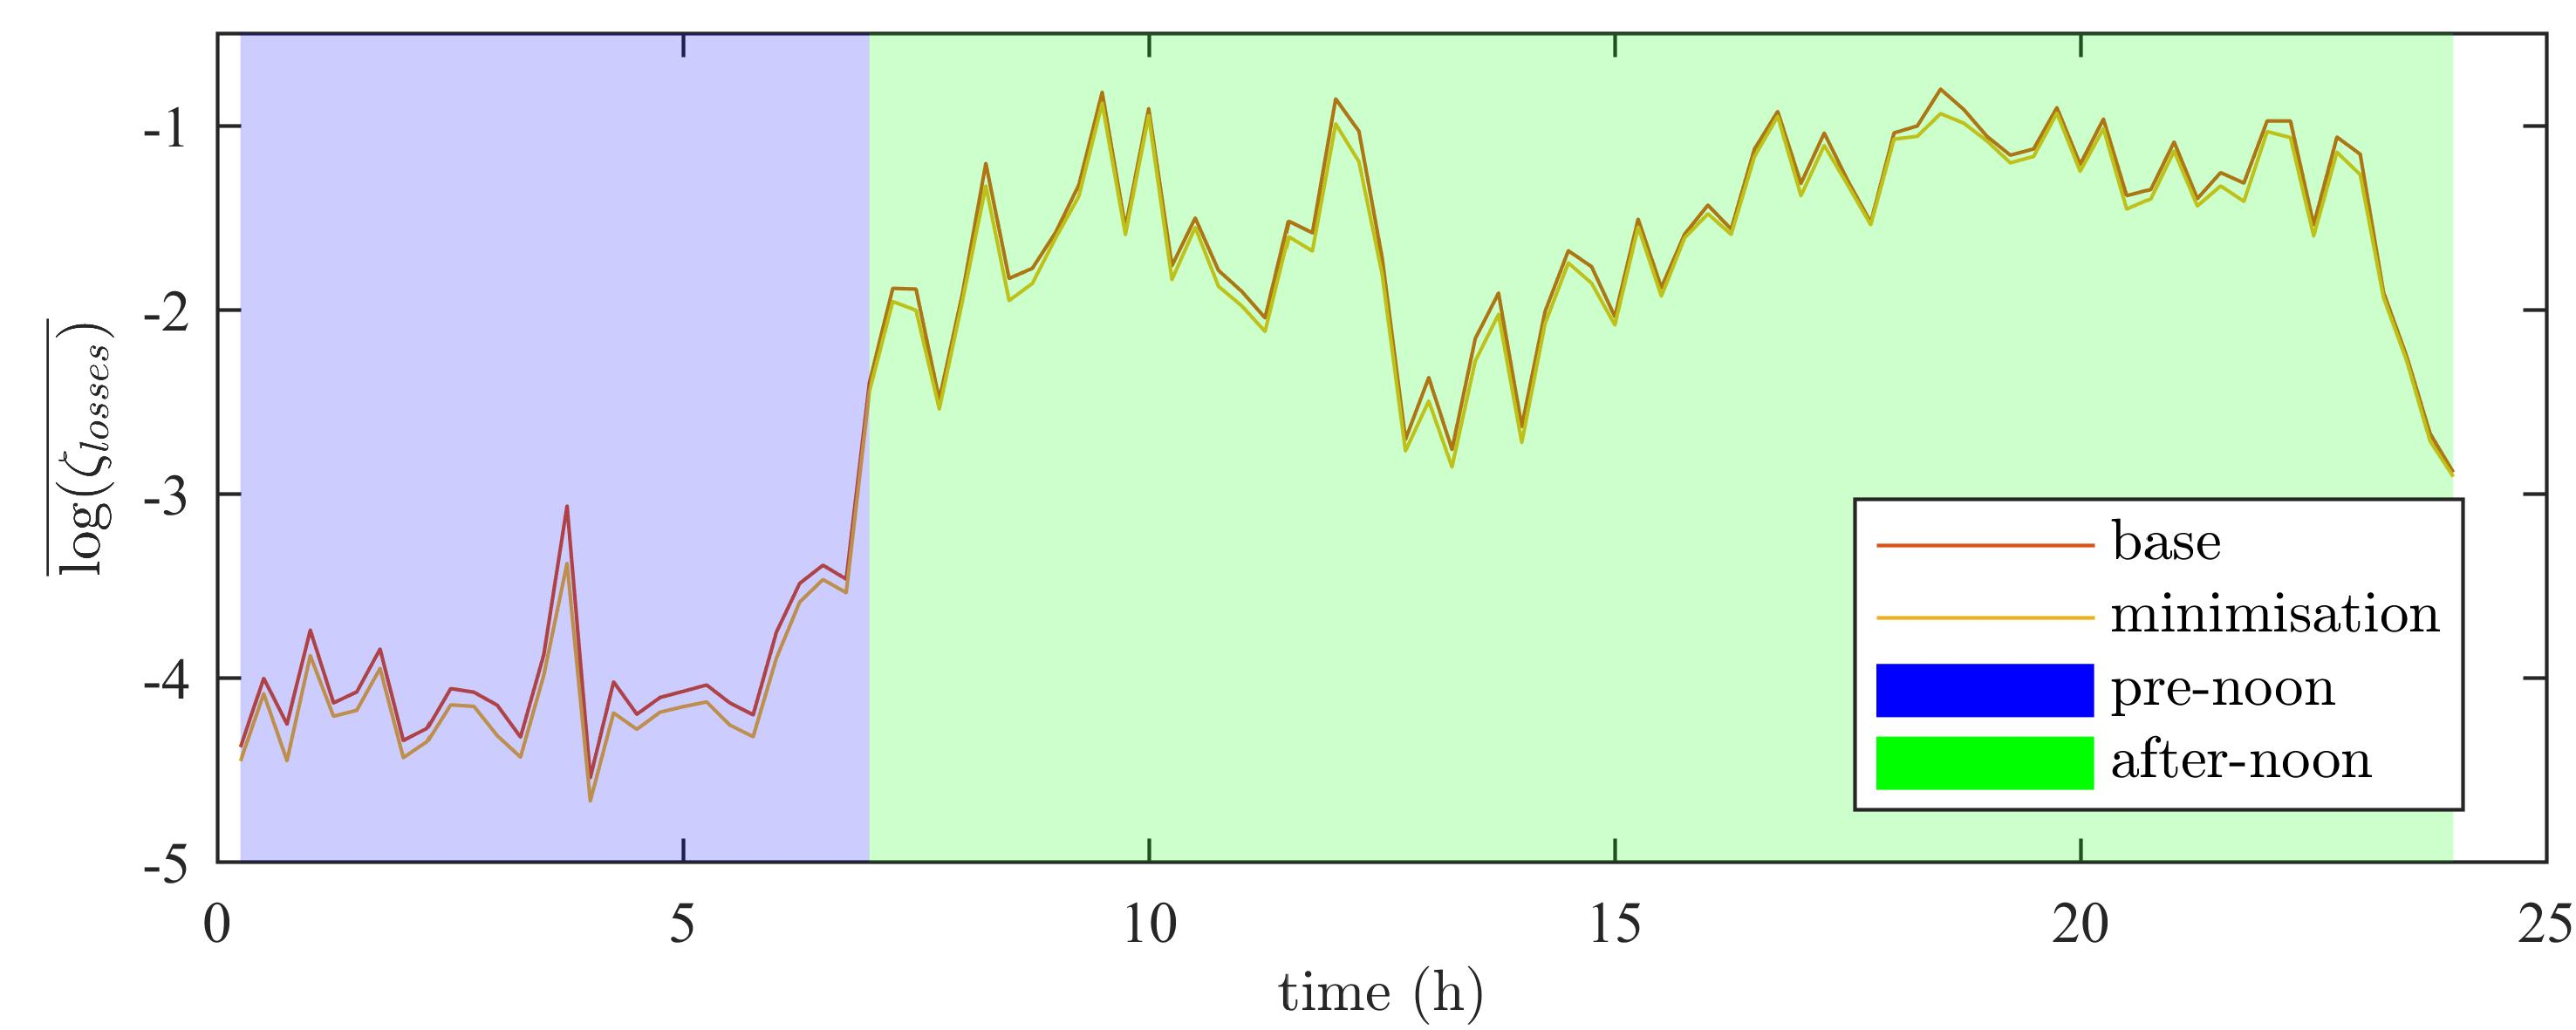
\includegraphics{_appendices/_a1/fig/averaged-log-cost-split}
	\caption{Splitting of the conditioned data into two stationary sections}
	\label{appx-a:ch1:fig:split-averaged-log-data}
\end{figure}

The preconditioned data in the two sections, that are highlighted in Figure~\ref{appx-a:ch1:fig:split-averaged-log-data}, are now compared by computing their difference.
Figure~\ref{appx-a:ch1:fig:split-averaged-log-data-difference} shows this difference.

\begin{figure}\centering
	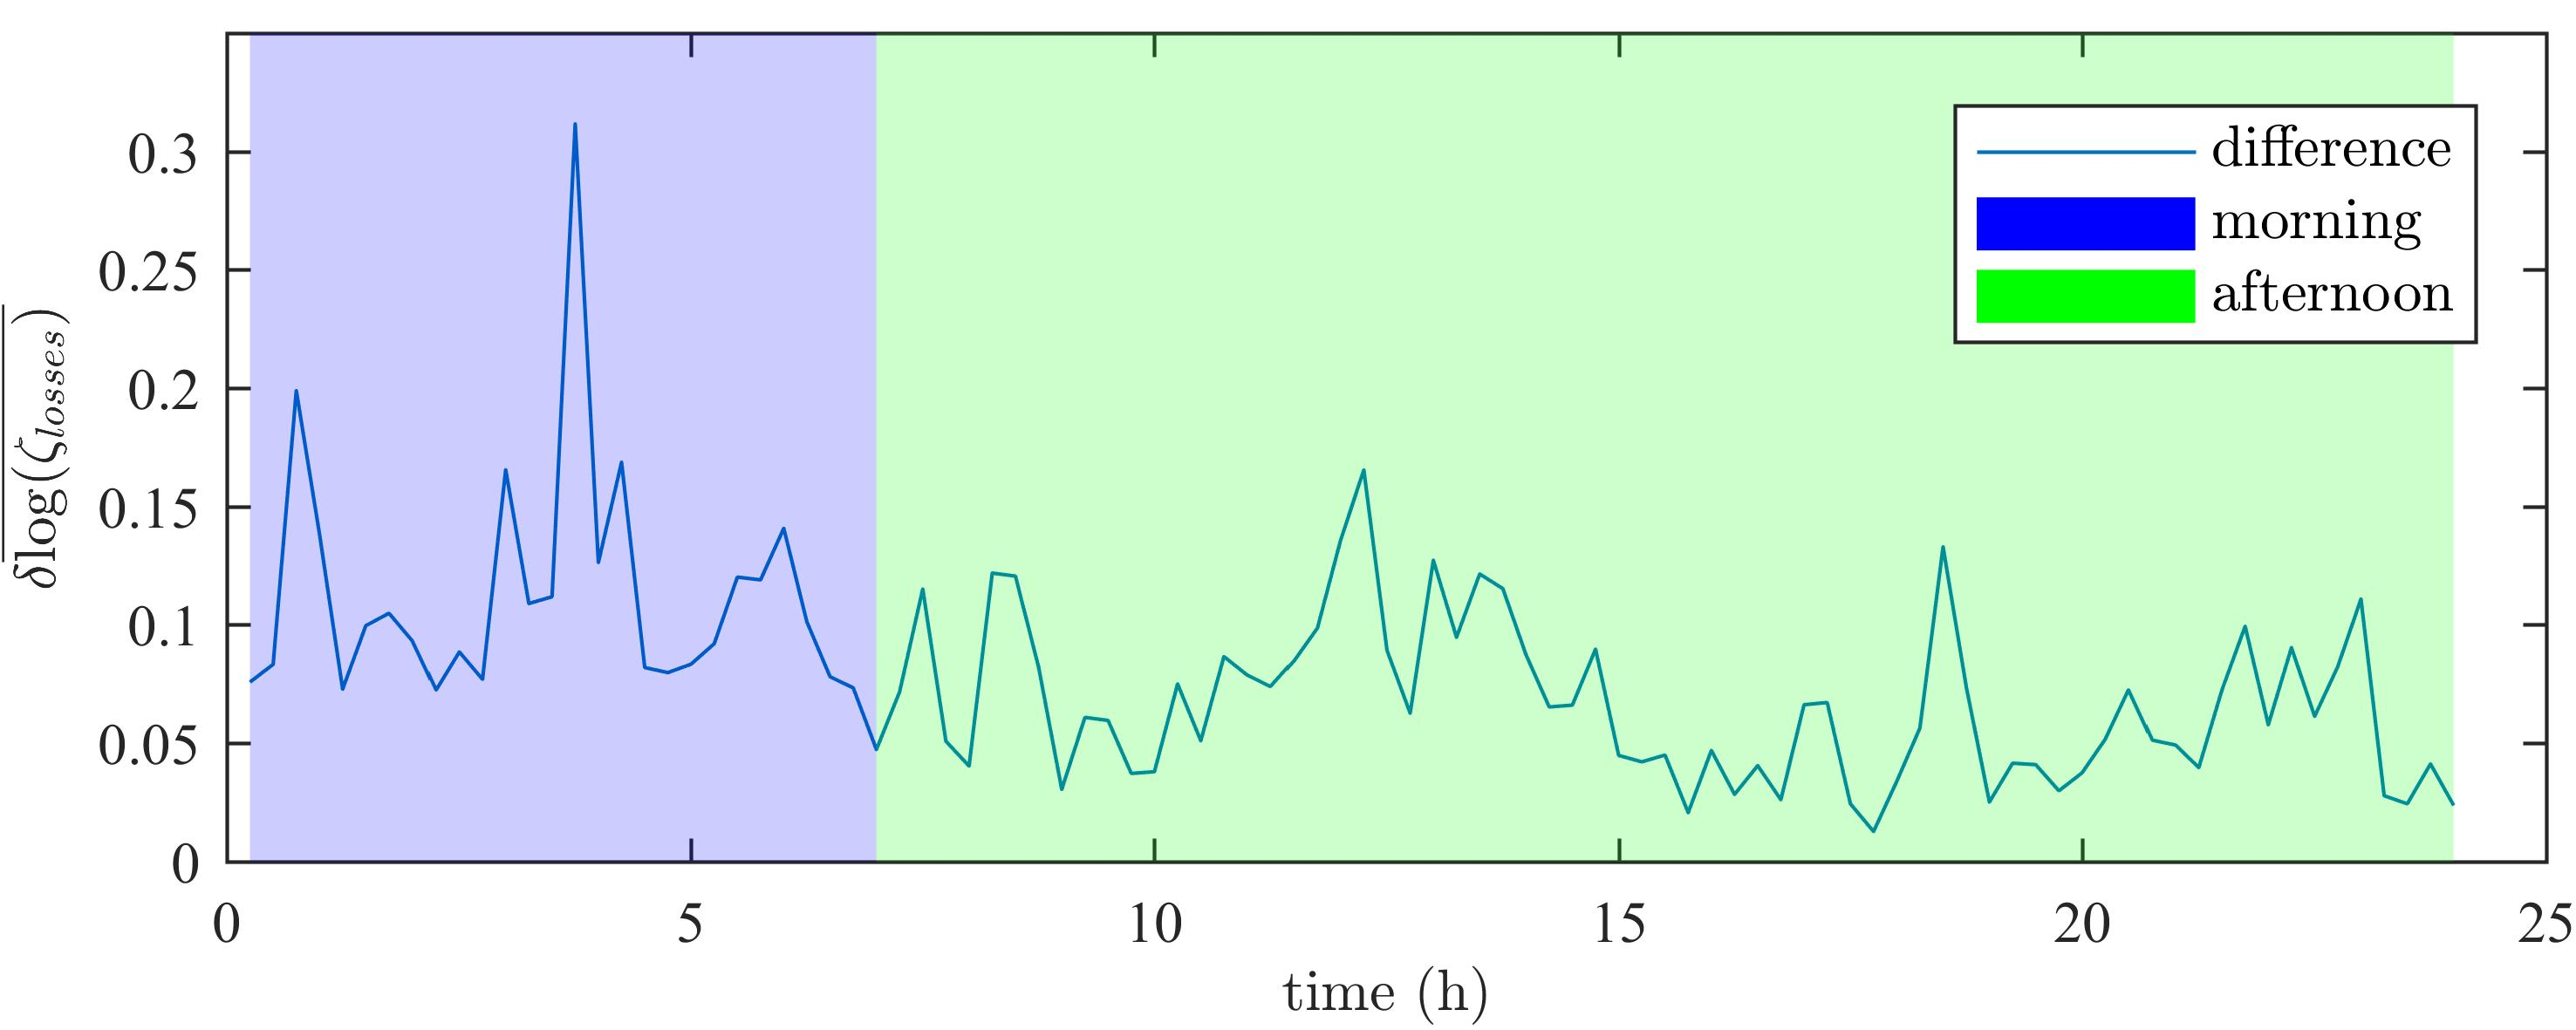
\includegraphics{_appendices/_a1/fig/averaged-log-cost-difference}
	\caption{Difference of the two pre-conditioned time-series.}
	\label{appx-a:ch1:fig:split-averaged-log-data-difference}
\end{figure}

This difference is now auto-correlated and to indicate if any ``self-dependence'' (i.e. indicating auto-regression) is still present in the data.
Results from both sections are shown in Figure~\ref{appx-a:ch1:fig:section-auto-correlation}

\begin{figure}\centering
	\subfloat[]{
		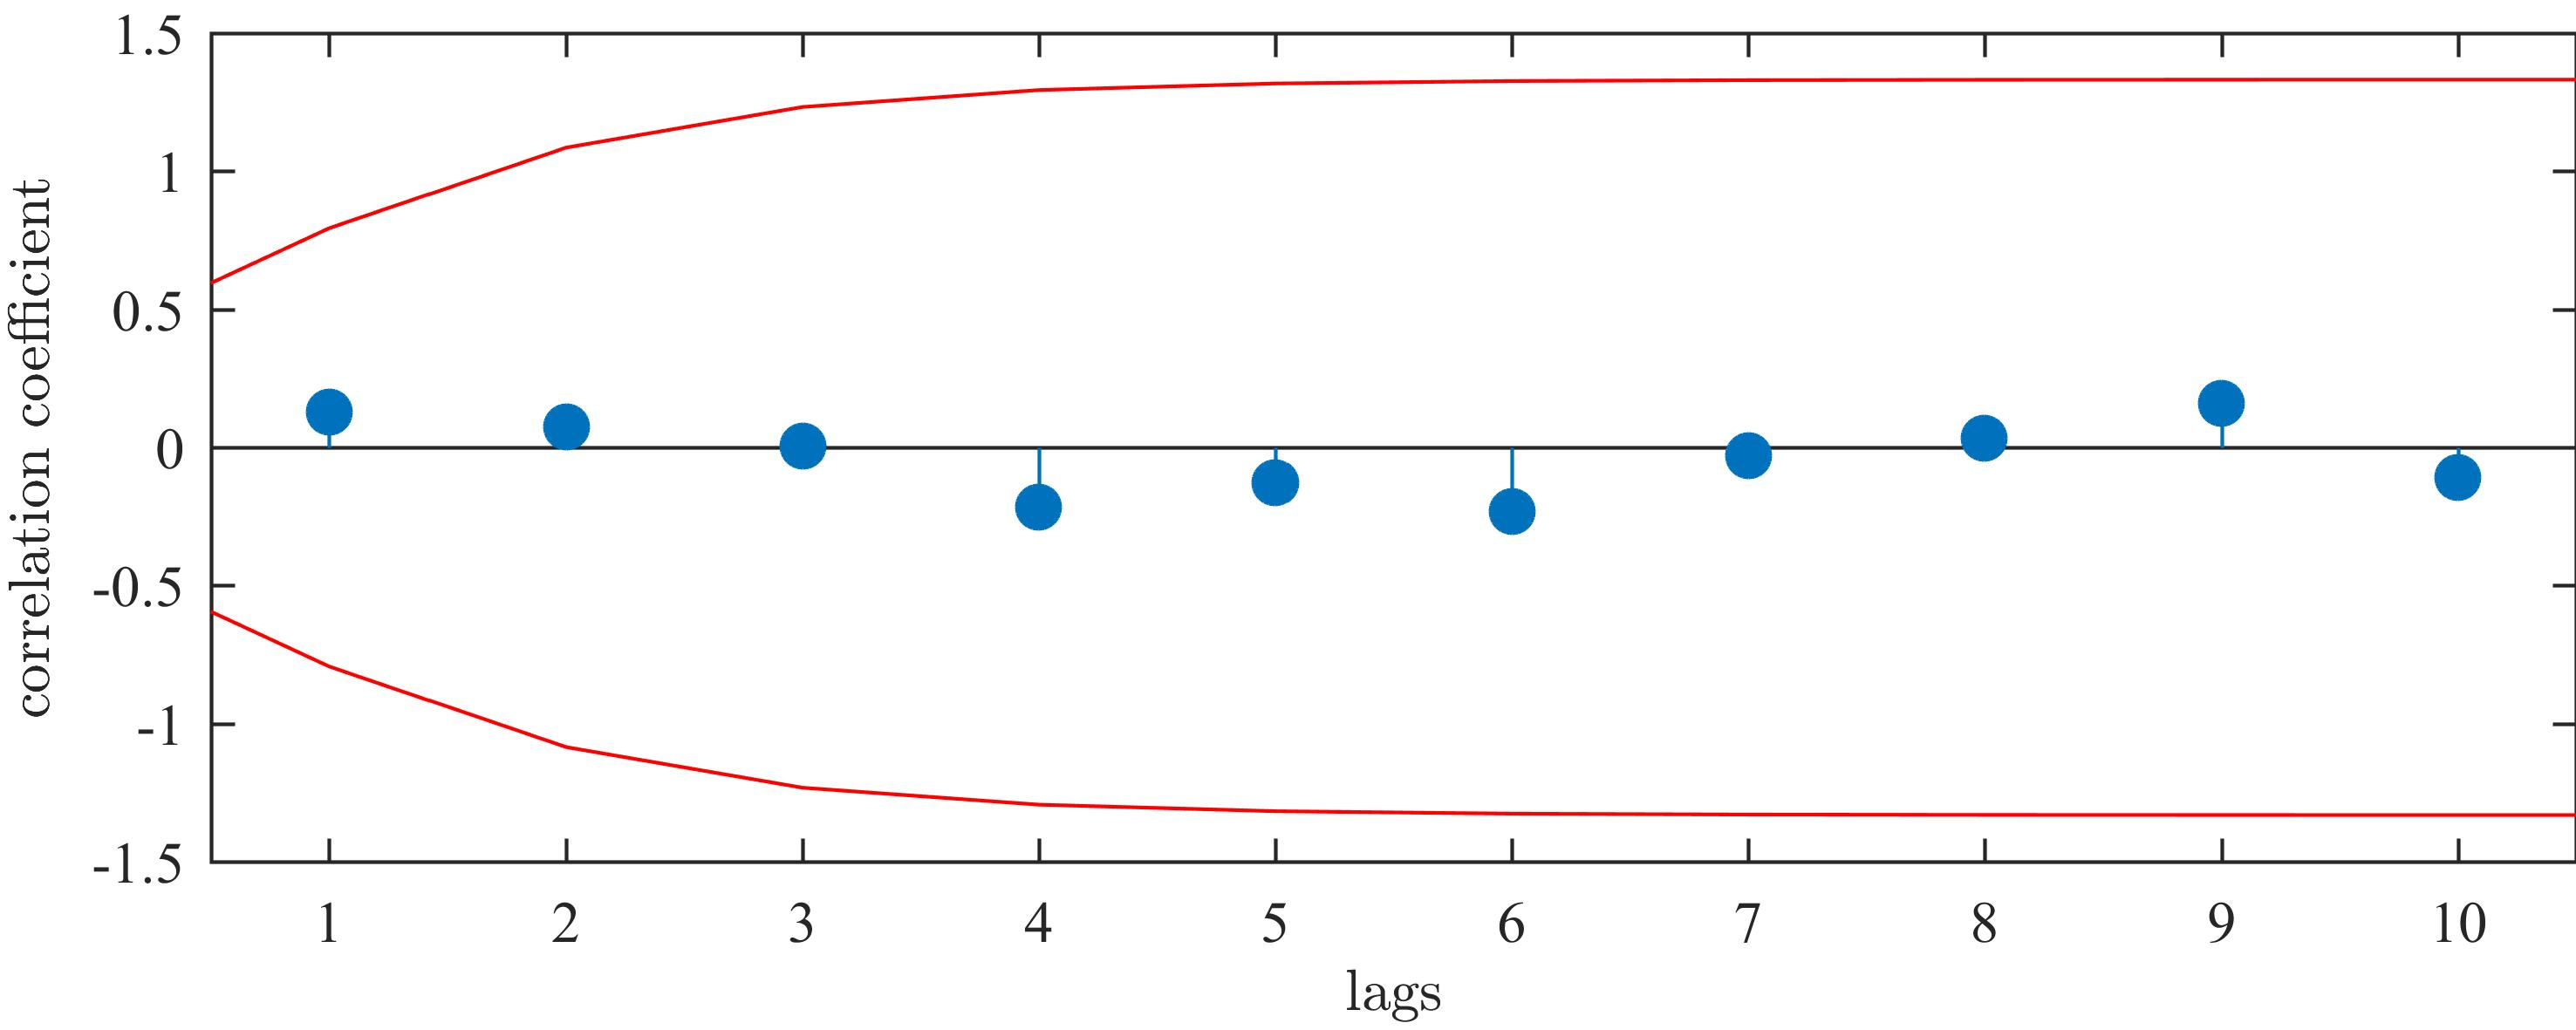
\includegraphics{_appendices/_a1/fig/autocorr_1}
		\label{appx-a:ch1:fig:section-auto-correlation-1}
	}\\
	\subfloat[]{
		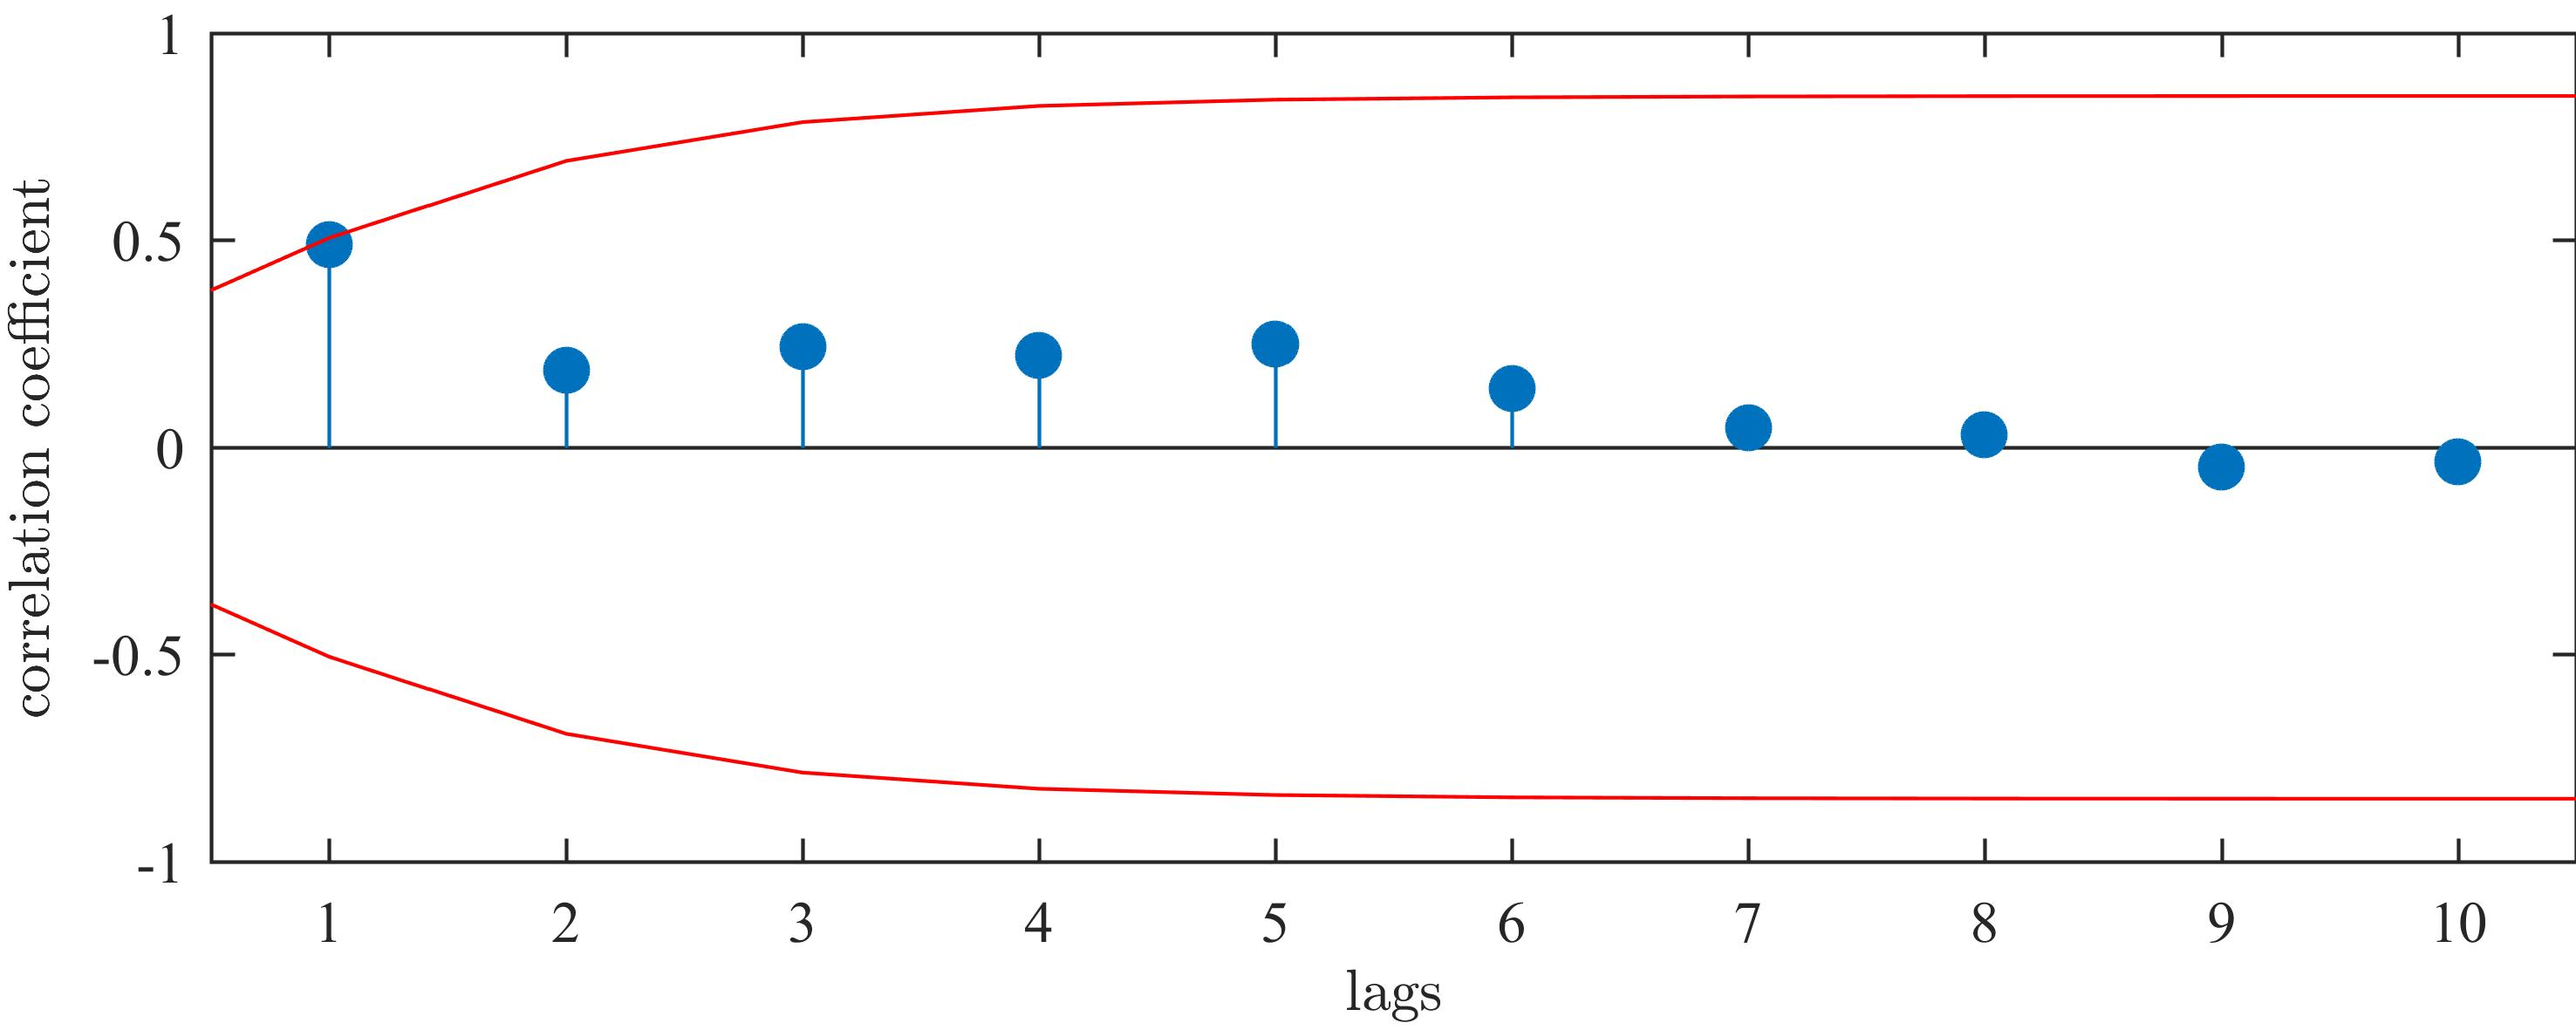
\includegraphics{_appendices/_a1/fig/autocorr_2}
		\label{appx-a:ch1:fig:section-auto-correlation-2}
	}
	\caption{Auto-correlation of signal for (\ref{appx-a:ch1:fig:section-auto-correlation-1}) morning and (\ref{appx-a:ch1:fig:section-auto-correlation-2}) afternoon sections}
	\label{appx-a:ch1:fig:section-auto-correlation}	
\end{figure}


Using the statistics package \textit{MINITAB}, the significance bounds are determined.
If any auto-correlation value lies outside this bound, then the data still contains significant self-dependence and must be re-conditioned.
In the case presented in Figure~\ref{appx-a:ch1:fig:section-auto-correlation} however, the auto-correlation indices lie within the bounds for all lags.
Therefore, the criteria for the $t$-test are met and the data can be assessed.
In this case, the $t$-test resulted in $p<0.001$, which is the same value that is used in the ``Probability Density Analysis'' Section~\ref{ch1:sec:results-and-discussion}.





